\chapter{Sniffer \& Portscanner}

\section{Introduzione}

Gli \textbf{\emph{Sniffer \& Port scanner}} sono argomenti interessanti ed importanti nell'ambito delle applicazioni di rete.\
Tuttavia, sono argomenti complessi e solitamente vengono trattati in seminari o corsi sulla sicurezza informatica.\
Ambiti di utilizzo:

\begin{itemize}
    \item \textbf{\emph{lecito}};
    \item \textbf{\emph{illecito}}.
\end{itemize}
Gli sniffer e i portscanner sono tipi di strumenti diametralmente opposti:
\begin{itemize}
    \item \textbf{passivi} (\emph{sniffer})
    \item \textbf{attivi} (\emph{port scanner})
\end{itemize}
\begin{figure}[H]
    \centering
    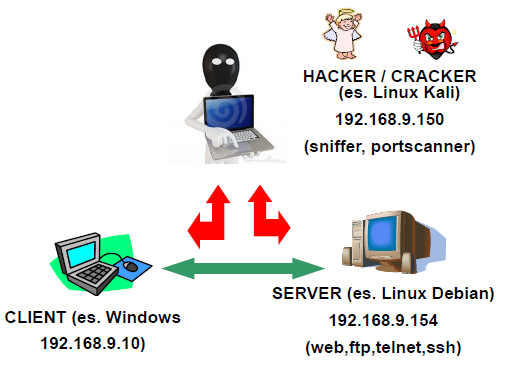
\includegraphics[width=0.8\textwidth]{immagini/Sniffer&portscanner.png}
    \caption*{Situazione tipica}
\end{figure}
Li vediamo in ambito \textbf{\emph{lecito}} (didattico, debug, risoluzione problemi, errori configurazione, ecc\dots).\
Esempi ``reali e/o pratici'':

\begin{itemize}
    \item sniffer:\ src/dst uguale server LAN laboratorio.
    \item sniffer:\ bittorrent e consumo banda notebook.
    \item sniffer/portscan:\ trojan o malware redirezione traffico uscita (web) o rete nascosta (botnet).
    \item portscan:\ installare un nuovo dispositivo (servizi attivi).
    \item sniffer/portscan:\ identificazione virus (es.\
          Conficker).
\end{itemize}

\begin{center}
    \textbf{Attenzione a cosa si fa!!}
\end{center}
\begin{itemize}
    \item Non si può attivare uno sniffer in una rete senza autorizzazione
          \begin{itemize}
              \item privacy, raccolta informazioni, normativa sul lavoro, ecc\dots
          \end{itemize}
    \item Non si può effettuare portscan liberamente contro qualsiasi obiettivo senza autorizzazione
          \begin{itemize}
              \item regolamento ISP, controlli \& IDS, risvolti legali, ecc\dots
          \end{itemize}
\end{itemize}

\section{Sniffer}

\subsubsection{Storia}

I programmi per il network tracing sono noti dalla fine degli anni '80.\
A quel tempo gli analizzatori per scopi commerciali non erano disponibili; il più famoso era il programma Sniffer, sviluppato da Network General.\
Il termine sniffing risale a tale programma.\


Sulle macchine Unix il programma tcpdump è stato sviluppato da Van Jacobsen, Leers e McCanne alla fine degli anni '80, questo programma e la libreria libpcap possono essere visti come i nonni di Wireshark.

All'inizio degli anni '90 erano disponibili molti analizzatori di pacchetti commerciali, la maggior parte di essi erano costosi e integrati nell'hardware.\


La situazione è cambiata alla fine degli anni '90 con lo sviluppo di ``Ethereal'' di Gerald Combs, questo programma è stato costruito sopra libpcap e la libreria GIMP Tool Kit (GTK), questo ha portato un analizzatore gratuito a molti sistemi operativi diversi.

\subsection{Cosa è uno sniffer?}

Uno \emph{sniffer} è un software per leggere ed analizzare il traffico di rete che arriva ad una certa macchina; si deve avere accesso alla rete locale.

Opera direttamente al livello di collegamento fisico della rete ethernet, quindi ai livelli 1 (fisico) e 2 (data link).\
È utile per scopi:
\begin{itemize}
    \item \textbf{leciti}:\ didattici, test, debug e monitoraggio (NIC guasta).
    \item \textbf{illeciti}:\ traffico non autorizzato, username/password, rootkit \& backdoor.
\end{itemize}
Si imposta l’interfaccia di rete in \textbf{\emph{modalità promiscua}} (cattura cioè anche il traffico non diretto alla propria scheda di rete):
\begin{itemize}
    \item ifconfig eth0 promisc
    \item ifconfig eth0 -promisc (ritorno modo funzionamento normale).
\end{itemize}
Deve essere eseguito con i privilegi di root (o amministratore).

\begin{figure}[H]
    \centering
    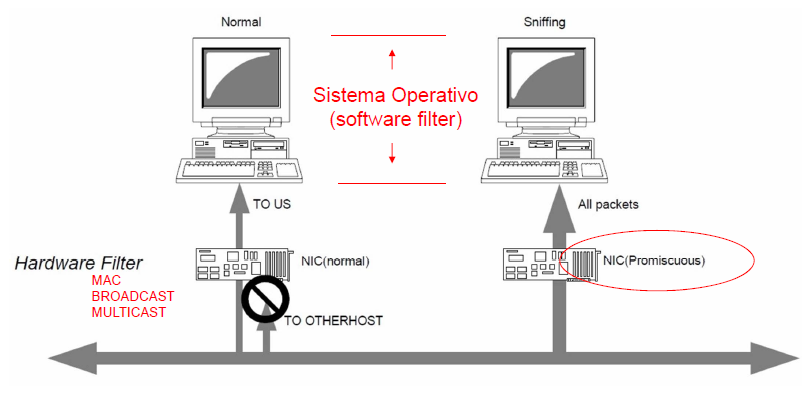
\includegraphics[width=\textwidth]{immagini/Promiscuous_mode.png}
    \caption*{Modalità promiscua}
\end{figure}

\begin{figure}[H]
    \centering
    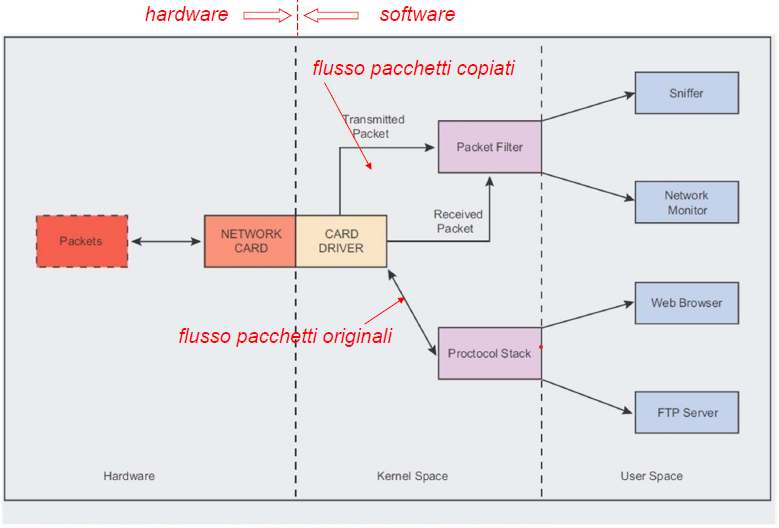
\includegraphics[width=0.8\textwidth]{immagini/Capture_process.png}
    \caption*{Elementi coinvolti nel processo di cattura}
\end{figure}
L’attività di sniffing (causa la copia dei pacchetti) è quindi onerosa dal punto di vista computazionale:

\begin{itemize}
    \item CPU
    \item memoria RAM
    \item spazio disco
    \item conseguente rallentamento attività di rete
\end{itemize}
Dipende dalla quantità di traffico da
analizzare:
\begin{itemize}
    \item possibile perdita di pacchetti (NIC o driver inadatti)
    \item Large Receive Offload (lro), Generic Receive Offload (gro)
          \begin{itemize}
              \item NIC riassembla i pacchetti prima di passarli al kernel
              \item problemi con alcuni sniffer evoluti (snort)
          \end{itemize}
\end{itemize}
Nell’ambito dello \emph{sniffing}, abbiamo dei problemi in ambienti di rete con gli \textbf{switch}.\
Uno \textbf{sniffer} deve poter ``vedere'' tutto il traffico che ci interessa.

\subsubsection{Switch Ethernet}

Ha un certo numero di porte Ethernet.\
Il traffico è veicolato \textbf{esclusivamente} fra le porte a cui sono connessi i dispositivi che lo generano e che devono riceverlo:
\begin{itemize}
    \item Sicurezza (proprio contro gli sniffer)
    \item Prestazioni (traffico esclusivamente tra mittente e destinatario)
\end{itemize}
Mano a mano che gli host generano traffico lo switch memorizza le associazioni ``MAC address source'' $\rightarrow$ ``porta''.\


Instrada i frame Ethernet esclusivamente verso la porta sulla quale lo switch ``vede'' il MAC address di destinazione.\
Replica del frame su tutte le porte (comportamento hub):
\begin{itemize}
    \item se il MAC address è quello di broadcast;
    \item se non è a lui noto.
\end{itemize}
\dots in una LAN ``\textbf{\emph{switchata}}'' esistono diverse soluzioni:
\begin{itemize}
    \item porta \textbf{MONITOR} o \textbf{SPAN} (\emph{Switch Port ANalyzer}) dove replicare il traffico delle porte interessate o tutto il traffico.
    \item un ``vecchio'' \textbf{HUB} (\emph{per reti non troppo veloci}).
    \item dispositivi \textbf{TAP} (\emph{Test Access Port}).
    \item \textbf{BRIDGE software}.
    \item \textbf{ARP cache Poisoning} (!!)
\end{itemize}
\begin{figure}[H]
    \centering
    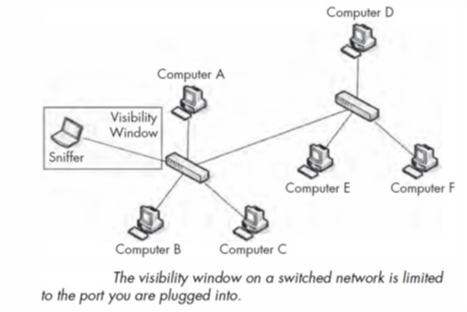
\includegraphics[width=0.6\textwidth]{immagini/sniffer_switch.png}
\end{figure}

\subsection{Come lavora uno sniffer?}

Il processo di packet-sniffing coinvolge hardware (NIC) \& software.\
Imposta la NIC in promiscuos mode; tutto il traffico viene catturato e passato al sistema operativo e alle applicazioni specifiche.\
Il funzionamento prevede 3 passaggi:
\begin{itemize}
    \item \emph{Raccolta}:\ sono raccolti i dati binary grezzi (raw).
    \item \emph{Conversione}:\ sono convertiti in forma leggibile (interpretabile), anche se solo a basso livello; molti tool a linea di comando si fermano qui (tcpdump).
    \item \emph{Analisi}:\ analisi approfondita ed elaborata dei dati raccolti; alcuni software evoluti agevolano l’analisi da parte dell’utente (wireshark).
\end{itemize}
In ambiente GNU/Linux si usano solitamente le librerie \textbf{libpcap} (\emph{Packet Capture}).\
In ambiente MS Windows le \emph{classiche} librerie \textbf{winpcap} o le \emph{nuove} \textbf{npcap}.

Si sfruttano le funzionalità chiamate \textbf{BPF} (Berkeley Packet Filter); permettono di specificare delle espressioni come filtro (\emph{poter selezionare solo il traffico di interesse}).\
Tali funzionalità sono fornite direttamente dalla libreria libpcap con sintassi generica (\emph{standard de-facto}); utilizzate con tutti gli sniffer (e anche molti IDS) che usano libpcap.\
Il file del traffico catturato (in formato .pcap) può quindi essere analizzato con software e strumenti diversi (tcpdump, wireshark, ecc).\
Il formato .pcap è di fatto uno standard.

\begin{figure}[H]
    \centering
    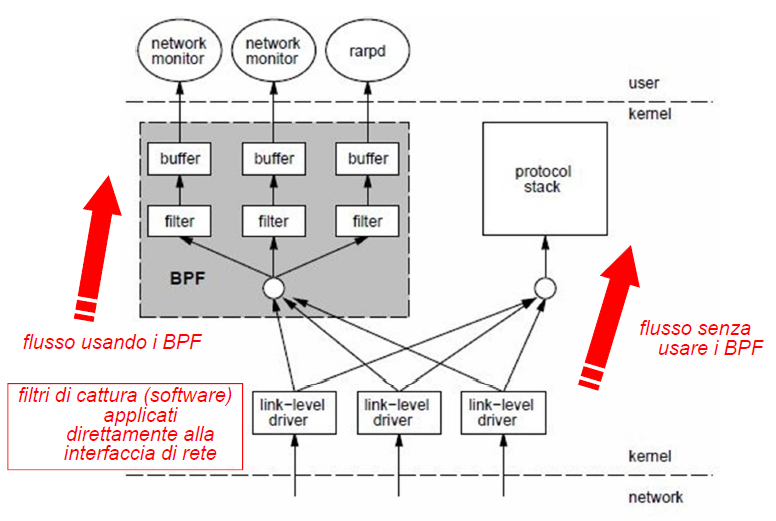
\includegraphics[width=0.7\textwidth]{immagini/BPF_overview.png}
    \caption*{BPF Overview}
\end{figure}

\begin{figure}[H]
    \centering
    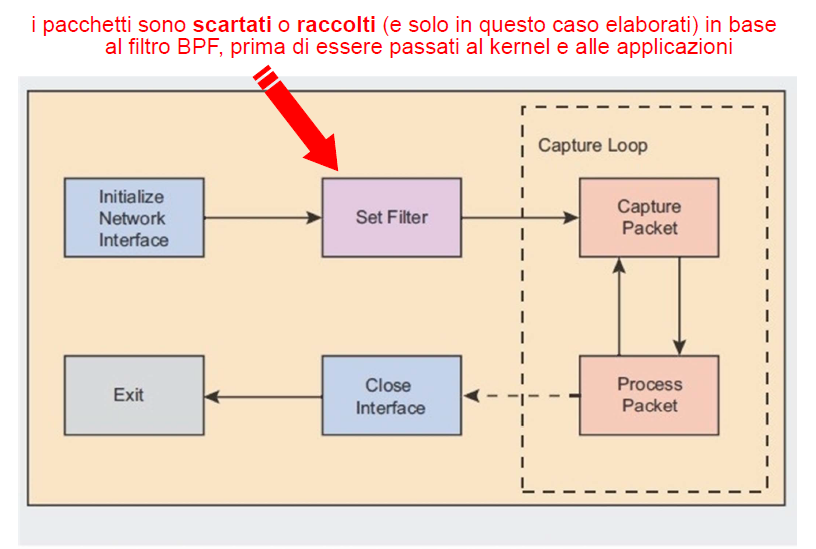
\includegraphics[width=0.9\textwidth]{immagini/pcap_flow.png}
    \caption*{Normal program flow of a pcap application}
\end{figure}

\subsubsection{Esempi di sniffer}

In ambiente GNU/Linux:
\begin{itemize}
    \item TCPDUMP
    \item suite WIRESHARK (TSHARK versione command line, DUMPCAP, EDITCAP)
    \item IPTRAF (network monitor)
    \item XPLICO (network forensic analysis tool)
    \item NGREP
    \item ETTERCAP (MiTM), NAST
    \item DSNIFF (password sniffer), P0F (fingerprint passivo)
    \item TCPKILL
    \item ETHERAPE (network monitor)
    \item NTOP (network monitor)
    \item SNORT (Network IDS)
\end{itemize}
In ambiente Microsoft Windows:
\begin{itemize}
    \item suite WIRESHARK (TSHARK versione command line, DUMPCAP, EDITCAP)
    \item WINDUMP (versione tcpdump per MS Windows)
    \item SATORI (fingerprint passivo)
    \item CAIN \& ABEL
    \item Microsoft MESSAGE ANALYZER (ex Microsoft NETWORK MONITOR):\ sfrutta driver a basso livello del Sistema Operativo MS Windows, spesso usato per sniffer WiFi $\rightarrow$ \textbf{dismesso/deprecato}
    \item RAWCAP, SMARTSNIFF (localhost,loopback)
\end{itemize}

\subsection{TCPDUMP}

\begin{itemize}
    \item In pratica è una interfaccia a riga di comando della libreria libpcap.\

    \item Permette di catturare il traffico di rete in tempo reale, di salvarlo su file (per una analisi successiva) e di rileggere file .pcap raccolti anche con software diversi.
\end{itemize}

\begin{table}[H]
    \centering
    \begin{tabular}{|l|m{28em}|}
        \hline
        Opzione  & Descrizione                                                                         \\\hline\hline
        -i iface & specifica un'interfaccia su cui ascoltare.                                          \\
        -w file  & scrive i pacchetti letti sul file \textbf{file}.                                    \\
        -r file  & legge i pacchetti dal file \textbf{file}.                                           \\
        -c count & legge esattamente \textbf{count} pacchetti.                                         \\
        -n       & non effettua la risoluzione degli indirizzi.                                        \\
        -p       & non porta l'interfaccia in modo promiscuo.                                          \\
        -t       & non stampa la temporizzazione dei pacchetti.                                        \\
        -v       & aumenta le informazioni stampate a video.                                           \\
        -q       & diminuisce le informazioni stampate a video.                                        \\
        -e       & stampa anche i dati relativi al protocollo di collegamento fisico (il MAC address). \\
        -F file  & usa il contenuto di \textbf{file} come filtro.                                      \\\hline
    \end{tabular}
\end{table}

\subsubsection{BPF (Berkley Packet Filter)}

Composti da quelle che si chiamano ``\emph{primitive}''; espressioni elementari che permettono di identificare una certa classe di traffico di rete.
\begin{center}
    \textbf{primitiva = qualificatore + identificatore}
\end{center}
Qualificatori:
\begin{itemize}
    \item \emph{di tipo}:\ host, net, port.
    \item \emph{di direzione}:\ src, dst, src or dst, src and dst.
    \item \emph{di protocollo}:\ ether, ip, ip6, arp, rarp, tcp, udp, icmp, \dots
\end{itemize}
TCPDUMP converte e compila ``al volo'' (\emph{runtime}) la sintassi BPF ad alto livello (primitive a livello utente) nel codice BPF a basso livello per la ``pseudo-machine'' (tcpdump -d).

Fondamentali in base a quantità di traffico (limitano dati da elaborare)
\begin{itemize}
    \item Security Onion
    \item Netsniff-NG (\emph{sniffer evoluto})
\end{itemize}

\begin{table}[H]
    \centering
    \begin{tabular}{|l|m{17em}|m{10em}|}
        \hline
        Qualifier & Description                                                     & Examples                       \\\hline \hline
        Type      & Identifies what the ID name or number refers to                 & host, net, port                \\
        Dir       & Specifies a transfer direction to or from the ID name or number & src, dst                       \\
        Proto     & Restricts the match to a particular protocol                    & ether, ip, tcp, udp, http, ftp \\\hline
    \end{tabular}
    \caption*{The BPF Qualifiers}

\end{table}
\begin{figure}[H]
    \centering
    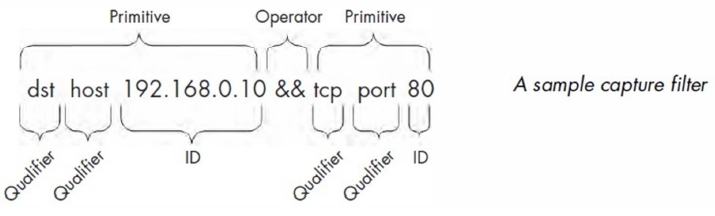
\includegraphics[width=0.7\textwidth]{immagini/capture_filter_ex.png}
\end{figure}

\subsubsection{Struttura di output di TCPDUMP}

L'output tcpdump fornisce per impostazione predefinita alcune informazioni di base su ciascun pacchetto.\
La formattazione di questo output varierà in base ai protocolli in uso, ma i formati più comuni sono:
\begin{itemize}
    \item TCP:

          [Timestamp] [Layer 3 Protocol] [Source IP].[Source Port]$>$[Destination IP].[Destination Port]:\ [TCP Flags], [TCP Sequence Number], [TCP Acknowledgment Number], [TCP Windows Size], [Data Length]
    \item UDP:

          [Timestamp] [Layer 3 Protocol] [Source IP].[Source Port]$>$[Destination IP].[Destination Port]:\ [Layer 4 Protocol], [Data Length]
\end{itemize}
Puoi forzare tcpdump a fornire più informazioni in questa riga di riepilogo aggiungendo il tag -v per aumentarne la verbosità.

\subsection{Wireshark}

Estremamente potente, dotato di interfaccia grafica che ne facilita l’utilizzo.\
Dispone di ``protocol dissector''; permetteno di effettuare
una ``dissezione'' (\emph{analisi}) dettagliata del traffico catturato.\
Permette di ricostruire il flusso di dati (stream) così da poter individuare i dati ``effettivamente'' catturati al livello di applicazione (email, pagine web, password, ecc\dots).

Crea statistiche e grafici dai dati elaborati.\
È possibile rileggere il traffico catturato in formato .pcap anche con strumenti diversi (es tcpdump).

Permette di usare i \textbf{filtri di cattura} BPF.\
Possiede dei \textbf{filtri di visualizzazione} per agevolare analisi.

È una suite di strumenti, esiste una versione testuale da linea di comando chiamato TSHARK.

\section{Port Scanner}

Software in grado di rilevare informazioni su un host (o una intera rete) e quali servizi sono attivi.\
Scansiona le porte (TCP e UDP) per identificare quali di esse sono utilizzate da un servizio.\
Può ``forzare'' a provocare certi tipi di risposta, al fine di raccogliere informazioni utili.

È uno strumento indispensabile per verificare in
maniera effettiva la \emph{propria} rete.\
Ê uno strumento di tipo attivo (a differenza di uno
sniffer).

In generale un port scanner genera traffico e ``confusione'' in una rete, quindi è potenzialmente identificabile.\
Usato per scopi \textbf{offensivi} (ricerca servizi vulnerabili
da attaccare), \textbf{indispensabile} per scopi di \textbf{difesa} (ricerca servizi vulnerabili o inutili da chiudere).

\subsubsection{Portsweep}

Tecnica di scansione simile al portscanning.\
Si effettua una scansione di uno o più host (o di una intera rete) alla ricerca della disponibilità di un singolo servizio (e/o una vulnerabilità) concentrandosi però su una singola porta.

Il portscannig, invece, effettua una scansione su diverse porte di diversi host (o una intera rete).\
Esempio:\ effettuare un portsweep degli host della nostra LAN sulla porta 3389 per individuarne versioni con problemi di sicurezza.
Le finalità sono le stesse del portscannig:
\begin{itemize}
    \item diagnostica
    \item attacco
\end{itemize}

\subsubsection{Individuazione/difesa}

La pratica del portscan è decisamente invasiva e può risultare ``pericolosa''; può essere identificata come un vero e proprio attacco informatico!!

La maggior parte dei sistemi di difesa prevedono dei metodi per identificarla; SNORT (uno dei Network IDS più utilizzati) prevede sia un preprocessore (sfportscan) che delle regole costruite ``ad-hoc'' al fine di identificare i portscan.

\subsection{NMAP}

È il più utilizzato per eseguire portscanning (comunque ne esistono altri).\
Estremamente flessibile ed ottimizzato:
\begin{itemize}
    \item esegue portscan più o meno invasivi e/o più o meno identificabili.
    \item rileva la presenza e tipologia di firewall.
    \item identifica caratteristiche e versione del sistema operativo e dei servizi remoti (fingerprint attivo).
    \item presenta report completi e dettagliati.
\end{itemize}
Prevede un proprio linguaggio di scripting (Nmap Scripting Engine - NSE) per automatizzare e migliorare le analisi.\
Scansiona intere reti in tempi brevissimi.\
Dotato anche di interfaccia grafica (ZENMAP).

\subsubsection{Funzionamento}

Per usufruire di tutte le sue funzionalità, si deve eseguire come amministratore (l’unico che può ``forgiare'' pacchetti ad-hoc).\
Si basa sul tipo di risposte ricevute previste dagli standard dei protocolli di rete.

Crea ad-hoc delle richieste (non sempre ``formalmente'' corrette) per generare delle risposte previste e predefinite.\
Sfrutta le peculiarità dei protocolli di rete (si addentra nei ``meandri'' del loro funzionamento).

Dalle risposte ricevute (e dal confronto con i suoi db interni) identifica tutta una serie di caratteristiche del sistema bersaglio.

Per default (\emph{escluso il Connect Scan -sT}) usa pacchetti minimali e non invasivi, quindi senza dati (vuoti):
\begin{itemize}
    \item il portscanning di solito ``non fa danni'' (a meno di bug del servizio remoto\dots); è la pratica del portscanning ritenuta dannosa/offensiva!
\end{itemize}
Cerca in questo modo di non lasciare tracce:
\begin{itemize}
    \item nei log dei servizi remoti.
    \item nei log del sistema operativo remoto:
          \begin{itemize}
              \item un pacchetto ``strano'' generato da nmap può causare un errore nello stack di rete remoto che può essere identificato:\ \emph{``May 15 11:28:57 server proftpd[3324] server:\ Fatal:\ unable to open incoming connection:\ Transport endpoint is not connected''}
          \end{itemize}
    \item è comunque impossibile prevedere tutte le possibili implementazioni dei servizi remoti (specialmente nel caso di servizi in UDP, dove i controlli sono demandati alla applicazione), quindi a volte qualche traccia risulta \dots
\end{itemize}

\subsubsection{Firewall}

\begin{itemize}
    \item DROP:\ il pacchetto ricevuto viene silenziosamente scartato (non viene inviata nessuna risposta al client).
    \item REJECT:\ il pacchetto ricevuto viene scartato ma viene prodotta una risposta verso il client:
          \begin{itemize}
              \item TCP:\ invio pacchetto RST.
              \item UDP:\ invio pacchetto ICMP ``Port Unreachable''.
              \item possibilità di personalizzare il tipo di risposta mediante la direttiva --reject-with \emph{TIPO\_PACCHETTO} (\emph{icmp-net-unreachable, icmp-portunreachable, icmp-proto-unreachable, ecc}\dots).
          \end{itemize}
\end{itemize}

\subsubsection{Portscan di default}

\begin{itemize}
    \item Come utente non privilegiato:CONNECT SCAN (-sT)
    \item Come utente amministratore (root):\ SYN SCAN (chiamato anche semi apertura o half-open) (-sS)
    \item A seguito della scansione, le porte possono risultare:
          \begin{itemize}
              \item OPEN:\ servizio attivo sulla porta ed accessibile.
              \item CLOSED:\ nessun servizio sulla porta.
              \item FILTERED:\ può essere attivo un servizio sulla porta ma la comunicazione è bloccata e non si è in grado di capire se OPEN o CLOSED.
              \item UNFILTERED:\ nel solo caso di TCP ACK Scan (-sA).
              \item OPEN| FILTERED:\ situazione indeterminata (nel caso di scanUDP, IP, protocol, FIN, NULL e Xmas).
              \item CLOSED|FILTERED:\ situazione indeterminata (nel solo caso di TCP Idle Scan -sI).
          \end{itemize}
\end{itemize}

\subsubsection{Connect scan (-sT)}

Effettua una serie di normali connessioni TCP (SYN$\rightarrow$, $\leftarrow$ SYN{\slash}ACK, ACK$\rightarrow$).\
Funzionamento:
\begin{itemize}
    \item porta aperta:\ si riceve una risposta dal demone attivo con successiva chiusura della connessione; porta OPEN.
    \item porta chiusa (senza firewall):\ si riceve in risposta una connessione abortita (invio di RST in risposta a connessione su porta chiusa, come previsto dallo stack TCP/IP); porta CLOSED.
    \item con firewall (DROP):\ non si riceve risposta, i pacchetti sono scartati dal firewall, quindi si ha un time out; porta FILTERED.
\end{itemize}
Questa modalità è facilmente individuabile dai log, causa apertura/chiusura di porte senza traffico effettivo.\
La dimensione del pacchetto SYN è quella normale; ci sono dati contenuti in ``options'' [mss, wscale, ecc\dots]

\subsubsection{SYN scan (-sS)}

È la modalità utilizzata di default (chiamata anche \emph{stealth mode}).\
Esegue la prima parte dell’apertura (semi-apertura) della connessione TCP (non completa la connessione iniziale, manca ACK finale dal client).\
Invio di un pacchetto SYN \textbf{\emph{creato da nmap}}:
\begin{itemize}
    \item porta aperta:\ si riceve in risposta SYN+ACK; OPEN
    \item porta chiusa:\ si riceve in risposta un RST/ACK; CLOSED
    \item Firewall (DROP):\ nessuna risposta; FILTERED
\end{itemize}
Non serve concludere la connessione da parte di nmap!

Se la porta è aperta e ricevo un SYN+ACK dal target, lo stack TCP del sistema dove si esegue nmap risponde con un RST poiché il SYN+ACK ricevuto dal target non corrisponde a nessun SYN iniziale iniziato da un processo del sistema.

NMAP usa ciò che si chiama ``\emph{RAW SOCKET}''.\
Crea artificialmente il SYN, invece di usare la systemcall \emph{connect()} del kernel (quindi, a differenza di -sT).\
Il pacchetto SYN (RAW SOCKET) creato da nmap è diverso (più piccolo) di un normale SYN; mancano dati in options (è
presente solo [mss]).

Non completando la connessione, il target in questo modo non si accorge di niente; questa scansione non lascia tracce sul target.\
Rilevabile però dalla maggior parte dei tool di sorveglianza (SNORT, Scanlogd, synlogger, ecc) e può essere bloccato da firewall che filtrano le nuove connessioni (SYN).

\subsubsection{Version detection (-sV)}

Tenta una connessione ai servizi trovati per determinarne la versione, in base alle risposte di questi ultimi:
\begin{itemize}
    \item banner ricevuto dal demone del servizio.
    \item altre informazioni distintive del servizio in ascolto.
\end{itemize}
Confronta le risposte con l’elenco presente nel file /usr/share/map/nmap-service-probes.

Nmap tenta la connessione ed aspetta circa 5 secondi una qualche risposta (tempo di rispondere se il servizio fosse impegnato).\
Può essere ``ingannato'' per eludere proprio i portscan:
\begin{itemize}
    \item modificando banner magari con quello di una versione senza bug.
    \item cambiando la porta di default (telnet sulla porta 22).
\end{itemize}
Nei log, questa scansione può lasciare tracce:
\begin{itemize}
    \item se è attivo sshd, in auth.log ritroviamo qualcosa tipo:\
          \begin{flushleft}
              ``\texttt{server sshd[2022]:\ Did not receive identification string from 192.168.9.151}''
          \end{flushleft}
    \item se è attivo un smtp server (es postfix), in mail.log ritroviamo qualcosa tipo:
          \begin{itemize}
              \item ``Apr 19 14:12:56 server postfix/smtpd[2463]:\ connect from unknown[192.168.9.151]''
              \item ``Apr 19 14:12:56 server postfix/smtpd[2463]:\ lost connection after CONNECT from unknown[192.168.9.151]''
              \item ``Apr 19 14:12:56 server postfix/smtpd[2463]:\ disconnect from unknown[192.168.9.151]''
          \end{itemize}
\end{itemize}
Potrebbe mandare in crash il servizio remoto (\emph{se non progettato correttamente\dots}).\
Generalmente viene individuata anche dai sistemi IDS.


\subsubsection{TCP/IP Fingerprint (-O)}

Analizzando le risposte ad una serie di pacchetti di prova, si cercano di identificare caratteristiche dello stack TCP/IP del TARGET, basandosi su una serie di risposte note (/usr/share/nmap/nmap-os-db).\


\textbf{\emph{Identifica il sistema operativo}}, in base alla TCP/IP fingerprint caratteristica di ogni OS.\
Identifica la predicibilità dei numeri di sequenza dello stack TCP (misura la difficoltà di creare pacchetti ad-hoc per inserirsi in una connessione).

\textbf{\emph{Identifica uptime}} del sistema.

\begin{figure}[H]
    \centering
    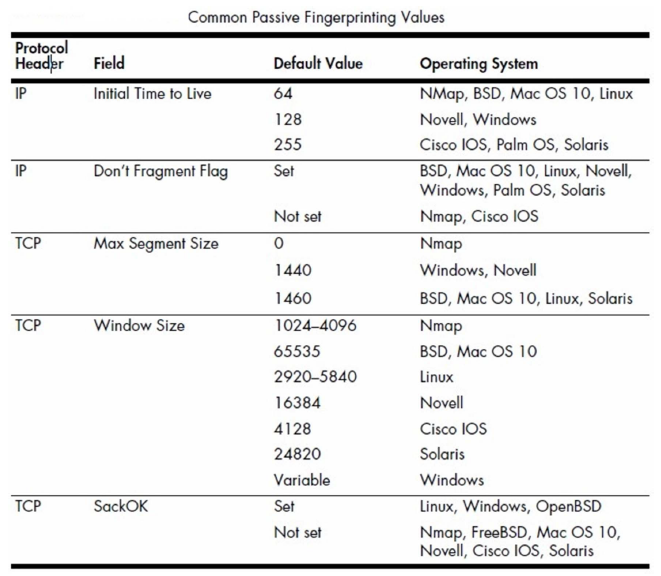
\includegraphics[width=0.8\textwidth]{immagini/Fingerprint_values.png}
\end{figure}

\begin{figure}[H]
    \centering
    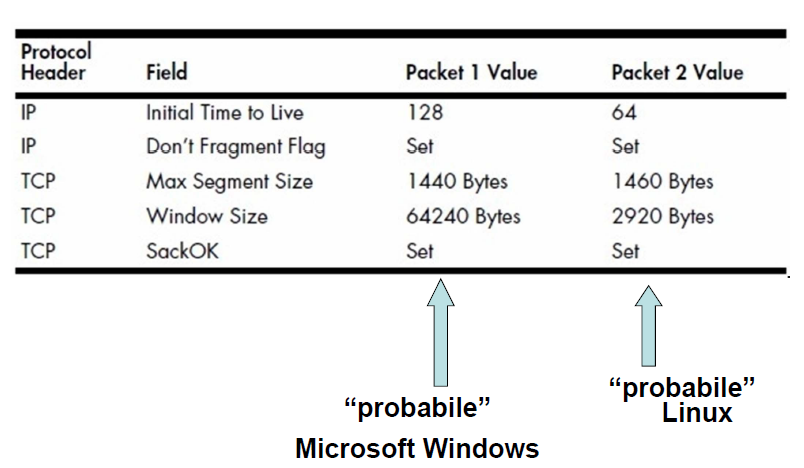
\includegraphics[width=0.8\textwidth]{immagini/Fingerprint_confronto.png}
    \caption*{Esempio di OS Fingerprint a confronto}
\end{figure}

\subsubsection{Curiosità}

È possibile riconoscere (con ragionevole certezza) il sistema operativo remoto molto banalmente osservando le risposte ad un semplice ping.\
Osservando il campo TTL della risposta:
\begin{itemize}
    \item Sistemi Microsoft:\ TTL inizia da 128
    \item Sistemi Linux:\ TTL inizia da 64
    \item Sistemi BSD:\ TTL inizia da 128
\end{itemize}
Non è casuale che i sistemi Microsoft e BSD forniscano le stesse tempistiche:\ Microsoft, ha costruito il proprio stack TCP/IP riprendendolo a piene mani dai sistemi BSD\dots
